\chapter{Detekce příjmu karbohydrátů}

Pro detekci příjmu karbohydrátů jsem měl k dispozici anonymizovaná data ze senzoru CGMS. Data obsahují naměřené a zadané hodnoty:
\begin{itemize}
\setlength\itemsep{0em}
\item Glukóza v krvi (BG)
\item Intersticiální glukóza (IST)
\item Bazální množství inzulinu
\item Bolus inzulinu
\item Příjem karbohydrátů (CHO)
\item Fyzická aktivita
\item Kvalita spánku
\item Počet kroků
\item Srdeční tep
\item Vodivost kůže
\item Teplota kůže
\item Teplota okolí
\end{itemize}

Pro detekci karbohydrátů jsem implementoval tyto 3 metody:
\begin{itemize}
\setlength\itemsep{0em}
\item Long short-term memory neuronová síť (kapitola \ref{ch:lstm})
\item Lineární a kvadratická diskriminační analýza (kapitola \ref{ch:lda_qda})
\item Detekce hran pomocí thresholdů 1. diference hodnot intersticiální glukózy \\(kapitola \ref{ch:threshold})
\end{itemize}

Programovací jazyk pro zpracování dat ze senzoru, návrh a vyhodnocení jednotlivých metod jsem zvolil Python. Python jsem zvolil pro jeho knihovny NumPy, pandas a SciPy pro zpracování a analýzu dat, matplotlib pro vykreslení dat a knihovny TensorFlow a Keras pro práci s neuronovými sítěmi. Přestože je Python interpretovaný jazyk a tudíž pomalý při zpracování velkého množství dat, tyto knihovny jsou implementovány v jazyce C a optimalizovány pro vysoký výkon. Doba zpracování dat je tak srovnatelná s kompilovanými jazyky.

Implementace do SmartCGMS je v jazyce C++.

\section{Příprava dat}

CGMS senzor posílá data ve formě signálů, které mají strukturu:
\begin{itemize}
\setlength\itemsep{0em}
\item Logical Clock
\item Device Time
\item Event Code
\item Signal
\item Info
\item Segment Id
\item Event Code Id
\item Device Id
\item Signal Id
\end{itemize}

Příklad signálů ze senzoru CGMS je v tabulce \ref{tab:cgms_data}

\begin{table}[H]
\caption{Signály ze CGMS}
\label{tab:cgms_data}
\centering
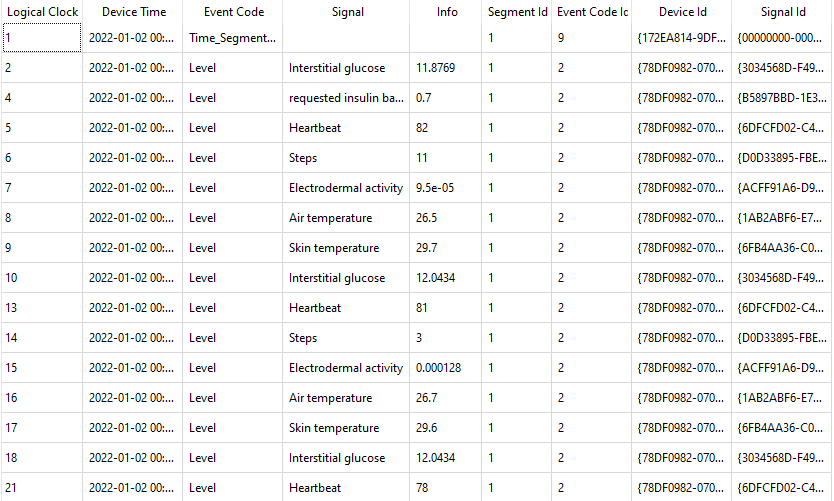
\includegraphics[width=1\textwidth]{img/cho/cgms_data.png}
\end{table}

Informaci pro následnou detekci v sobě nesou sloupce Device Time (čas měření), Signal (typ signálu) a Info (hodnota). Ty jsem extrahoval do dvourozměrné tabulky, kde řádky jsou čas měření a sloupce jednotlivé typy signálů.
Data intersticiální glukózy jsem interpoloval Akima spline \citep{cho.akima}, z níž jsem získal chybějící hodnoty a derivace 1. 2. a 3. řádu. Pro vyhlazení hodnot intersticiální glukózy jsem použil Savitzky-Golay filtr \citep{cho.savgol} řádu 3 s velikostí okna 21. Jelikož různé typy signálu nejsou měřeny ve stejný okamžik, řádky jsem seskupil podle sloupce intersticiální glukózy, která je měřena v pětiminutových intervalech.

V grafech na obrázku \ref{fig:48h_dataset} jsou transformovaná data naměřená senzorem CGMS za 48 hodin. Na prvním grafu jsou hodnoty Intersticiální glukózy a její vyhlazení Savitzky-Golay filtrem. Druhý graf znázorňuje zadanou bazální dávku inzulinu, bolusy, příjem karbohydrátů a fyzickou aktivitu. Na posledním grafu jsou zbylé měřené hodnoty.

\begin{figure}[H]
\caption{Data ze CGMS}
\label{fig:48h_dataset}
\centering
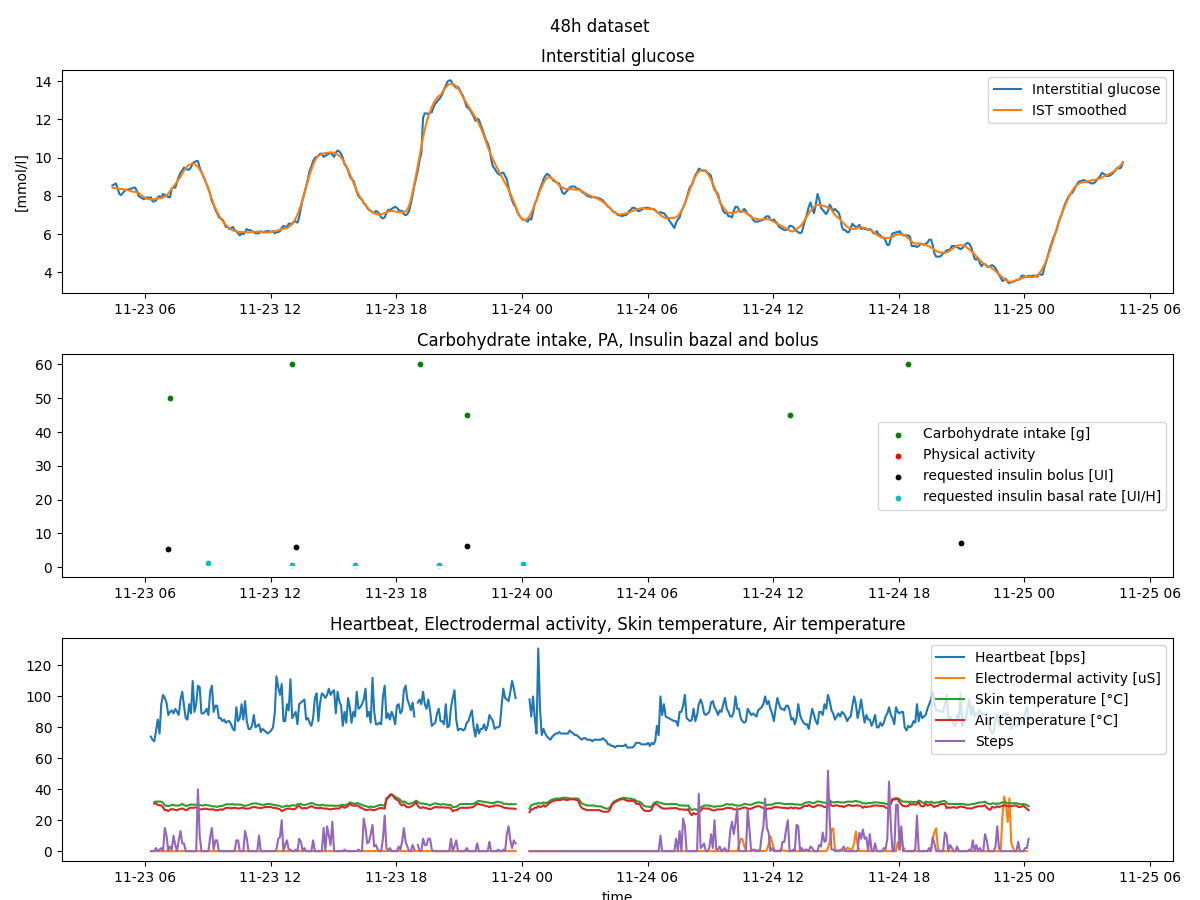
\includegraphics[width=1\textwidth]{img/cho/48h_dataset.png}
\end{figure}

\subsubsection{Spuštění}
Script pro transponaci dat se spustí zavoláním funkce:
\begin{verbatim}
load_log(patientID)
\end{verbatim}
ze souboru \texttt{load\_log.py}, kdy \textit{patientID} je ID pacienta. Logy musí být umístěny v adresáři data/. Pro spuštění transponace dat z více logů se zavolá funkce:
\begin{verbatim}
load_log_all(patientIDs)
\end{verbatim}
kdy \textit{patientIDs} je pole ID logů, které chceme transponovat. Transponovaná data jsou uložena do .csv souboru \textit{patientID-transposed.csv}.

Načtení a modifikace transponovaných dat se spustí voláním:
\begin{verbatim}
load_data(patientID, from_file, fill_missing, smooth,
           derivation, norm, verbose, graphs, analyze)
\end{verbatim}
ze souboru \texttt{load\_data.py}, potažmo
\begin{verbatim}
load_data_all(patientIDs, from_file, fill_missing, smooth,
                derivation, norm, verbose, graphs, analyze)
\end{verbatim}
pro načtení několika souborů. \textit{PatientID} je ID pacienta, \textit{from\_file} určuje zda se načtou již modifikovaná data nebo se spustí úprava transponovaných dat z logu. Parametr \textit{fill\_missing} určuje zda se mají nahradit chybějící hodnoty měření (\texttt{''} nenahrazuje se, 'akima' pro interpolaci Akima spline nebo 'mean' pro průměrnou hodnotu). Parametr \textit{smooth} určuje způsob filtrace ('savgol' pro Savitzky-Golay filter). Parametr \textit{derivation} určuje způsob výpočtu derivací ('akima' pro derivace Akima spline, 'gradient' pro numpy gradient, 'manual' pro výpočet diference). Parametr \textit{norm} říká, zda chceme data normalizovat ('std' normalizace směrodatnou odchylkou na interval <-1;1>, 'minmax' standardizace rozpětím na interval <0;1>). Parametr \textit{verbose} je pro vypsání průběhu zpracování dat, \textit{graph} zobrazí modifikovaná data v grafech a \textit{analyze} spustí analýzu dat z knihovny \textit{sweetviz}. Modifikovaná data jsou uložena do .csv souboru \textit{patientID-modified.csv}.


\section{Rekurentní neuronové sítě}
\label{ch:lstm}

Rekurentní neuronové sítě jsou vhodné pro predikci sekvenčních dat (například časové řady). Vyznačují se tím, že si předávají informaci o předchozím stavu (aktivaci skryté vrstvy):

$H_{t}=\sigma (W_{h}H_{t-1}+W_{x}X_{t}+b)$

\noindent kde $W$ jsou váhy a $b$ je bias. Neurony, které takto uchovávají svůj stav, se nazývají buňky. Riziko RNN spočívá v náchylnosti vzniku jevu označovaného jako mizející nebo explodující gradient vznikajícího při zpětné propagaci, kdy hodnoty exponenciálně klesají nebo rostou. To je z důvodu, že se chyba propaguje přes všechny iterace. Tento problém eliminuje long short-term memory nebo gated recurrent unit neuronová síť.

\begin{figure}[H]
\caption{Rekurentní neuronová síť}
\label{fig:rnn}
\centering
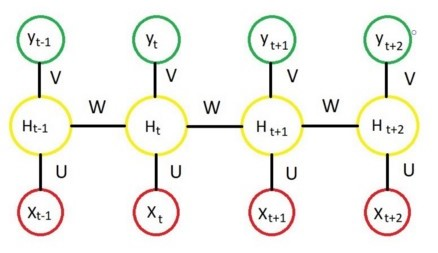
\includegraphics[width=0.7\textwidth]{img/cho/rnn.jpeg}\\
\textit{Zdroj: https://medium.com/}
\end{figure}

\subsection{Long short-term memory}

Long short-term memory neuronová síť (LSTM) je speciální případ rekurentní neuronové sítě. V každé iteraci si buňka uchovává dodatečnou informaci nazvanou \textit{memory}. 

Nejprve se ze vstupního vektoru $X_{t}$ a stavu předchozí buňky $H_{t-1}$ spočte Forget gate $f_{t}$, Candidate layer $\bar{C}_{t}$ Input gate $I_{t}$ a Output gate $O_{t}$ \citep{cho.lstm}:

$f_{t}=\sigma(X_{t} \otimes U_{f}+H_{t-1} \otimes W_{f})$\\\indent
$\bar{C}_{t}=tanh(X_{t} \otimes U_{c}+H_{t-1} \otimes W_{c})$\\\indent
$I_{t}=\sigma(X_{t} \otimes U_{i}+H_{t-1} \otimes W_{i})$\\\indent
$O_{t}=\sigma(X_{t} \otimes U_{u}+H_{t-1} \otimes W_{u})$

\noindent kde $W$ a $U$ jsou váhové vektory. Následně se spočte \textit{memory} prvek $C_{t}$:

$C_{t}=f_{t} \otimes C_{t-1} \oplus I_{t} \otimes \bar{C}_{t}$

\noindent a výstupní stav $H_{t}$:

$H_{t}=O_{t} \otimes tanh(C_{t})$

Diagram LSTM buňky je na obrázku \ref{fig:lstm_cell}.

\begin{figure}[H]
\caption{LSTM buňka}
\label{fig:lstm_cell}
\centering
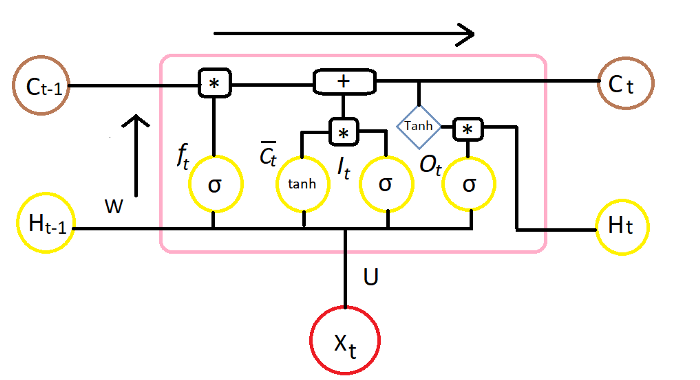
\includegraphics[width=1\textwidth]{img/cho/lstm_cell.png}
\textit{Zdroj: https://medium.com/}
\end{figure}

\subsection{Gated recurrent unit}

Gated recurrent unit neuronová síť (GRU) využívá Update gate $z_{t}$ a Reset gate $r_{t}$. Ty určují která informace bude propagována na výstup. Mohou tak vytěžit relevantní informace. Update a reset gate se spočte \citep{cho.gru}:

$z_{t}=\sigma(W_{z}x_{t} + U_{z}h_{t-1})$\\\indent
$r_{t}=\sigma(W_{r}x_{t} + U_{r}h_{t-1})$

\noindent kde $W$ a $U$ jsou váhové vektory. Následně se spočte relevantí informace z předchozího stavu $\bar{h}_{t}$:

$\bar{h}_{t}=tanh(W_{h}x_{t} + U_{h}(r_{t} \otimes h_{t-1}))$

\noindent a výstupní stav $h_{t}$:

$h_{t}=z_{t} \otimes h_{t-1} + (1-z_{t}) \otimes \bar{h}_{t}$

Diagram GRU buňky je na obrázku \ref{fig:gru_cell}.

\begin{figure}[H]
\caption{GRU buňka}
\label{fig:gru_cell}
\centering
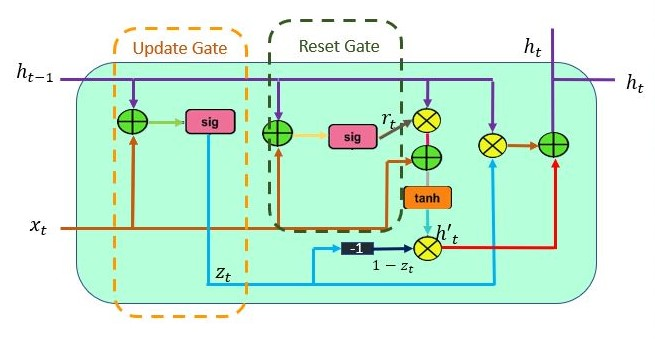
\includegraphics[width=1\textwidth]{img/cho/gru_cell.jpg}
\textit{Zdroj: https://www.pluralsight.com/}
\end{figure}

\subsection{Model}

Pro detekci karbohydrátů jsem sestavil sekvenční keras\footnote{Keras je nadstavba nad knihovnou TensorFlow pro neuronové sítě} model se čtyřmi vrstvami:
\begin{itemize}
\setlength\itemsep{0em}
\item Obousměrná LSTM nebo GRU
\item Dropout(0,5)
\item Dense(128)
\item Dense(1)
\end{itemize}

První vrstvou je rekurentní neuronová síť. Ta může být buď LSTM nebo GRU. Tato vrstva má 128 neuronů a dropout 0,2. Vstupem vrstvy je časové okno N vstupních prvků velikosti W. Tvar vstupních dat je WxN:

$\begin{bmatrix}
X^{1}_{1} & X^{2}_{1} & ... & X^{N}_{1}\\
X^{1}_{2} & X^{2}_{2} & ... & X^{N}_{2}\\
... & ... & ... & ...\\
X^{1}_{W} & X^{2}_{W} & ... & X^{N}_{W}
\end{bmatrix}$

Dropout vrstva s \textit{rate=0,2} náhodně nastaví některé vstupy na nulu v poměru 0,2. Nevynulované vstupy jsou škálovány 1/(1-rate), takže součet všech vstupů je nezměněn. To zabrání přetrénování neuronové sítě. Droupout vrstva je aplikována pouze při trénování sítě. První Dense vrstva (propojení neuronů formou každý s každým) má 128 neuronů, aktivační funkce je \textit{relu}. Druhá Dense vrstva s jedním neuronem je výstupní.

Jako ztrátová funkce je použita střední kvadratická chyba (MeanSquaredError), optimalizační algoritmus je Adam. Z datasetu je 80 \% dat použito pro trénování a 20 \% pro validaci. Data jsou do neuronové sítě dávkována v dávkách o velikosti 64. Jelikož se jedná o časovou řadu, data se nepromíchávají.

\subsubsection{Spuštění}

Trénování neuronové sítě se spustí voláním funkce:
\begin{verbatim}
lstm(df, headers, label, type, width, epochs)
\end{verbatim}
ze souboru \texttt{cho\_detection.py}, kde \textit{df} je pandas dataframe modifikovaných dat, \textit{headers} je pole názvů sloupců vstupních dat, \textit{label} je predikovaná třída, \textit{type} je LSTM nebo GRU, \textit{width} je velikost okna a \textit{epochs} je počet epoch, kolikrát má proběhnout trénovací cyklus.

Natrénovaný model se uloží do souboru \texttt{model/[patientID]\_keras\_model.h5} a následně se exportuje do souboru \texttt{model/[patientID]\_fdeep\_model.h5}, který používá C++ knihovna frugally-deep (viz kapitola \ref{ch:implementace_scgms}).

\subsubsection{Výsledky}

Pro detekci karbohydrátů jsem jako vstupní prvky zvolil vyhlazená data intersticiální glukózy, jejich derivaci 1. řádu a minuty normalizované na interval <0;1>. Velikost okna je 24 (tj. 2 hodiny). Predikovaná třída je množství zadaných karbohydrátů. Tyto hodnoty jsou pro účel trénování rozkopírovány po dobu dvou hodin od času zadání. Neuronová síť je trénovaná ve 200 epochách.

Výstupem jsou predikované odhady karbohydrátů. Pro detekci příjmu karbohydrátů určíme threshold. Pakliže množství karbohydrátů predikovaných neuronovou sítí je větší než tento threshold, je detekováno jídlo. Threshold je pro každého pacienta jiný.

\textbf{//TODO}

\section{Lineární a kvadratická diskriminační analýza}
\label{ch:lda_qda}

Diskriminační analýzu jsem se rozhodl implementovat vzhledem k vysoké úspěšnosti a malému zpoždění, které dosáhli \citet{analyzaCHO.LDA} v článku \textbf{Pattern Recognition Reveals Characteristic Postprandial Glucose Changes: Non-Individualized Meal Detection in Diabetes Mellitus Type 1} (kapitola \ref{ch:analyzaCHO:lda}).

\subsection{Teorie}
Diskriminační analýza slouží k rozdělení prvků do konečného počtu tříd na základě lineární kombinace charakteristických prvků. Pro klasifikaci potřebujeme znát posteriory tříd \textbf{P(Y|X)}. Pravděpodobnostní model \textbf{P(X|y=k)} pro každou třídu \textbf{k} lineární a kvadratické diskriminační analýzy je dán vícerozměrnou Gaussovo distribucí \citep{cho.book.lda}:

\scalebox{1.2}{$P(X|y=k)=\frac{1}{(2\pi)^{p/2}|\sum_{k}|^{\frac{1}{2}}}e^{-\frac{1}{2}(x-\mu_{k})^{T}\sum^{-1}_{k}(x-\mu _{k})}$}\\\\
kde \textbf{p} je počet prvků. Pro predikci je pak použito Bayesovo rozhodovací pravidlo \citep{cho.book.lda}:

\scalebox{1.2}{$P(y=k|x)=\frac{P(x|y=k)P(y=k)}{P(x)}=\frac{P(x|y=k)P(y=k)}{\sum_{l}{P(x|y=l)P(y=l)}}$}\\\\
kdy hledáme třídu s maximálním posteriorem.

Logaritmus posterioru pro kvadratickou diskriminační analýzu (QDA) je \citep{cho.book.lda}:

$P(y=k|x)=-\frac{1}{2}log|\sum_{k}|-\frac{1}{2}(x-\mu_{k})^{T}\sum^{-1}_{k}(x-\mu_{k})+logP(y=k)$\\\\
Predikovaná třída je ta, která má maximální logaritmický posterior.

Lineární diskriminační analýza (LDA) je speciální případ QDA, kdy předpokládáme, že třídy mají stejnou kovarianční matici. Logaritmus posterioru je pak vyjádřen \citep{cho.scikit.lda}:

$P(y=k|x)=-\frac{1}{2}(x-\mu_{k})^{T}\sum^{-1}(x-\mu_{k})+logP(y=k)$\\

Vstupem diskriminační analýzy může být buď množina prvků pro daný časový okamžik nebo časové okno jednoho prvku. Predikované třídy jsou příjem/nepříjem karbohydrátů. Ty dostaneme převedením sloupce karbohydrátů na booleanovskou proměnnou (0 je false, cokoli větší než 0 je true).

\subsection{Množina prvků}

Nejčastějším vstupem diskriminační analýzy je množina charakteristických prvků $X_{i}$. V tomto případě se diskriminační analýza snaží rozdělit prostor tak, aby odlišila jednotlivé třídy (viz obrázek \ref{fig:lda}).

\begin{figure}[H]
\caption{Rozdělení prostoru lineární diskriminační analýzou dvou prvků}
\label{fig:lda}
\centering
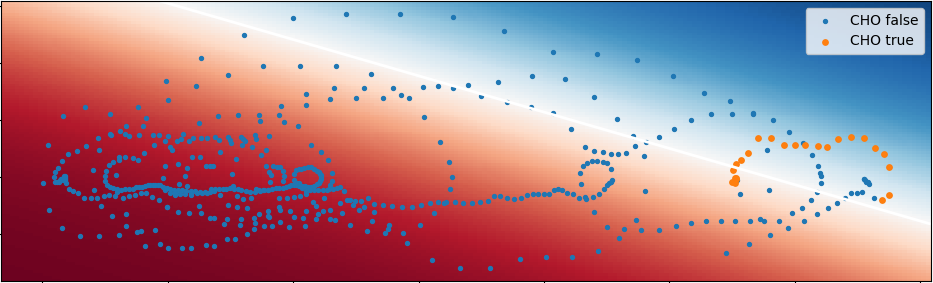
\includegraphics[width=1\textwidth]{img/cho/lda2.png}
\end{figure}

\subsubsection{Spuštění}

Trénování LDA a QDA pro množinu prvků se spustí voláním funkce:
\begin{verbatim}
lda(df, headers)
\end{verbatim}
ze souboru \texttt{cho\_detection.py}, kde \textit{df} je pandas dataframe modifikovaných dat, \textit{headers} je pole názvu sloupců vstupních dat.

\subsubsection{Výsledky}

\textbf{//TODO}

\subsection{Časové okno}

V případě časového okna muže být na vstupu pouze jediný prvek. To je dáno tím, že vstupem diskriminační analýzy je jedno-dimenzionální pole dat. Vstupní data mají tvar:

$\begin{bmatrix}
X_{i-W} & X_{i-W-1} & ... & X_{i-1} & X_{i}
\end{bmatrix}$

\noindent kde W je velikost časového okna.

\subsubsection{Spuštění}

Trénování LDA a QDA pro časové okno se spustí voláním funkce:
\begin{verbatim}
lda_window(df, header, width)
\end{verbatim}
ze souboru \texttt{cho\_detection.py}, kde \textit{df} je pandas dataframe modifikovaných dat, \textit{header} je název sloupce vstupních dat a \textit{width} je velikost okna.

\subsubsection{Výsledky}

\textbf{//TODO}


\section{Detekce hran průběhu intersticiální glukózy}
\label{ch:threshold}

Tato metoda detekuje vzestupné a klesající hrany průběhu intersticiální glukózy pomocí thresholdů první diference měřených hodnot intersticiální glukózy.

Derivace funkce $f'(x)$ v bodě $x$ je směrnicí tečny funkce $f(x)$ v daném bodě. Pakliže je funkce $f(x)$ v bodě $x$ rostoucí, je její směrnice tečny v bodě $x$ kladná. Pokud je $f(x)$ klesající, její směrnice tečny je v daném místě záporná. Velikost derivace v bodě $x$ pak udává velikost změny $f(x)$, neboli říká, jak strmě funkce stoupá či klesá. Derivace funkce $f(x)$ v bodě $x_{1}$ můžeme vyjádřit jako:

\scalebox{1.2}{$f'(x) = \frac{d}{dx}f(x) = \lim_{x \to x_{0}} \frac{f(x)-f(x_{0})}{x-x_{0}}$}

Jelikož data ze senzoru CGMS jsou diskrétní, můžeme derivaci nahradit rovnicí první diference. Pro data intersticiální glukózy tak dostáváme vztah:

\scalebox{1.2}{$\Delta IST = \frac{IST_{t} - IST_{t-1}}{\Delta t}$}

Naměřená data intersticiální glukózy mohou být zatížena šumem a případně i dočasnými výchylkami hodnot glukózy. Každá taková výchylka pak má značný vliv na hodnotu derivace. Z toho důvodu je potřeba data před výpočtem vyhladit. Pro vyhlazení dat byl zvolen digitální Savitzky-Golay filtr. Každá podmnožina $2m+1$ prvků je vzorkována na polynom stupně $p (p\leq 2m)$ ve smyslu nejmenších čtverců \citep{cho.savgol}. Pro vyhlazení dat intersticiální glukózy jsem zvolil polynom stupně 3 a velikost podmnožiny 21. Vyhlazená data vidíme v grafu na obrázku \ref{fig:savgol}.

\begin{figure}[H]
\caption{Vyhlazená data intersticiální glukózy}
\label{fig:savgol}
\centering
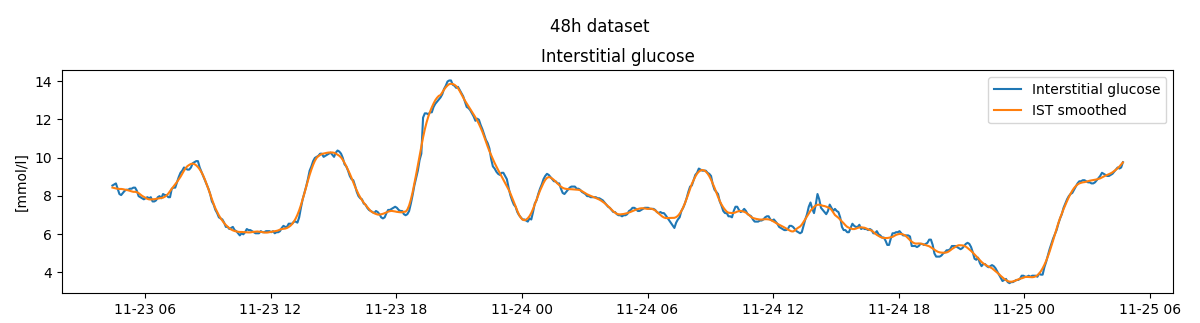
\includegraphics[width=1\textwidth]{img/cho/savgol.png}
\end{figure}

Následně se data ohodnotí. Pokud $\Delta IST$ překročí určitý threshold $th_{i}$, přiřadí se váha $w_{i}$. Takových dvojic thresholdů a vah může být libovolné množství. Experimentálně byla zjištěna kombinace thresholdů $th=[0.0125, 0.018]$ a vah $w=[2.25, 3]$.

Samotné ohodnocení podle thresholdů zachytí jakýkoli jednorázový větší výkyv v datech intersticiální glukózy. Jelikož příjem karbohydrátů se projevuje zvýšením glykémie v řádu desítek minut až hodin, chceme znát vývoj křivky intersticiální glukózy v čase. Z toho důvodu pro kladně ohodnocená data zvýšíme ohodnocení v případě, že předchozí hodnoty vykazují vzrůstající trend po dobu dvou hodin nazpět (tj. 24 hodnot, data jsou vzorkována po pěti minutách). Získáme tak aktivační funkci pro rostoucí hrany.
\begin{verbatim}
if activation[i] > 2:
  for j in range(24):
    if activation[i-j] >= 2+0.2*j:
      activation[i] += 0.1*j
\end{verbatim}
Pro klesající hrany použijeme stejný postup, ale se záporným ohodnocením.

\subsubsection{Spuštění}

Detekce hran průběhu intersticiální glukózy se spustí voláním funkce:
\begin{verbatim}
threshold(df, th, weight)
\end{verbatim}
ze souboru \texttt{cho\_detection.py}, kde \textit{df} je pandas dataframe modifikovaných dat (load\_data musí být spuštěno s parametry smooth='savgol', derivation='difference', norm=''), \textit{th} je pole thresholdů a \textit{weight} je pole vah o stejné délce. Funkce vrací hodnoty aktivační funkce.

\subsubsection{Výsledky}
V grafu na obrázku \ref{fig:hrany} je ukázka detekce hran. Červeně je aktivace vzestupné hrany, modře aktivace sestupné hrany posunuté. Počátek sestupné hrany je posunut na úrověň poslední hodnoty aktivace vzestupné hrany. Mezi vzestupnou a sestupnou hranou je vždy několik hodnot, kdy byla hladina intersticiální glukózy vyrovnaná.

\begin{figure}[H]
\caption{Detekované hrany průběhu intersticiální glukózy}
\label{fig:hrany}
\centering
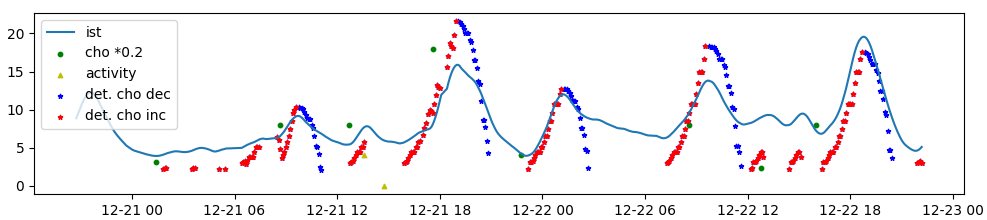
\includegraphics[width=1\textwidth]{img/cho/hrany.png}
\end{figure}

Jídlo je detekováno, pakliže aktivační funkce vzestupné hrany je větší než zvolený threshold. Nízký threshold detekuje většinu jídel, ale také může detekovat výkyvy nesouvisející s příjmem karbohydrátů. Naopak vysoce zvolený threshold nebude detekovat menší jídla. Řešením je použití více thresholdů pro stanovení pravděpodobnosti jídla.

\textbf{//TODO}

%Výsoký počet falešně pozitivních výsledků se mi částečně podařilo redukovat při implementaci do SmartCGMS.


\section{Implementace do SmartCGMS}
\label{ch:implementace_scgms}

Do SmartCGMS jsem implementoval filtr pro detekci karbohydrátů pomocí detekce hran průběhu intersticiální glukózy a pomocí rekurentních neuronových sítí. Dále bylo potřeba implementoval Savitzky-Golay filtr pro vyhlazení dat a evaluační filtr. Vytvořené filtry jsou zkompilovány do knihovny \texttt{cho\_detection.dll}.

Filtry implementují rozhraní \textit{scgms::IFilter} a \textit{refcnt::IReferenced}. Při vytvoření instance filtru se volá metoda \textit{Configure}, která slouží pro nastavení filtru (typicky přečtení a nastavení konfiguračních parametrů). Metoda \textit{Execute} je volána pokaždé, když přijde signál od předchozího filtru. Tato metoda vykonává požadovanou funkcionalitu. Původní událost se na závěr zpravidla posílá dalšímu filtru. Současně se musí zaregistrovat descriptor nového filtru, který definuje ID filtru, název a konfigurační parametry, a případně i descriptor nového signálu. Vytvořená dynamická knihovna musí exportovat funkce \textit{do\_create\_filter}, \textit{do\_get\_filter\_descriptors} a \textit{do\_get\_signal\_descriptors}.

Data mohou být rozdělena do časových segmentů dle měření. V takovém případě filtry pracují s každým segmentem zvlášť. Rozdělení do segmentů je realizováno pomocí mapy, kdy klíčem je ID segmentu.

Implementované algoritmy pracují s daty v určitém časovém okně. Pro tyto účely jsem vytvořil vlastní spojový seznam na principu klouzavého okénka \textbf{swl}. Ten dědí od \textit{std::deque}, které umožňuje vkládání prvků z obou stran i indexaci. konstruktor má jeden parametr určující velikost okna. Při vložení nadlimitního prvků se odebere prvek z druhého konce seznamu.

\textbf{Savitzky-Golay} filtr počítá vyhlazená data intersticiální glukózy. Výstupem je \textbf{IST smoothed} signál.

\textbf{CHO detection} filtr počítá aktivační funkci a detekci karbohydrátů. To je implementováno rekurentní neuronovou sítí nebo detekcí hran průběhu intersticiální glukózy. Filtr posílá dva signály. \textbf{Activation} signál je výstup použitého algoritmu a \textbf{CHO probability} udávající detekovaný příjem (1 - nižší pravděpodobnost, 2 - vyšší pravděpodobnost).

Rekurentní neuronová síť využívá natrénovaného keras modelu. Ten je možné použít v C++ pomocí knihovny frugally-deep \citep{cho.frugally}. Model je nutné konvertovat pomocí skriptu \texttt{keras\_export/convert\_model.py}, který je součástí frugally-deep knihovny. Podporované sítě jsou LSTM i GRU. Příklad konfigurace s GRU je v konfiguračním souboru \texttt{setup\_gru.ini} (viz příloha B).
 
V případě detekce hran jsou nastaveny 2 thresholdy. Nižší pro brzkou detekci, která ale může detekovat výkyvy nesouvisející s příjmem jídla. Vyšší threshold je potvrzovací, kdy existuje vysoká pravděpodobnost příjmu karbohydrátů. Detekce je pouze pro vzestupnou hranu. Potvrzení může být i pomocí rekurentní neuronové sítě. Příklad konfigurace thresholdů je v konfiguračním souboru \texttt{setup\_th.ini} (viz příloha B).

\textbf{Evaluate} filtr vyhodnocuje úspěšnost detekce. Pravdivě pozitivní (TP) jsou hodnoty, kdy je jídlo detekováno (hodnota detekce alespoň 1) do dvou hodin od jeho zadání pacientem. Pokud je hodnota detekce 2, je jídlo bráno jako potvrzeno. Pakliže jídlo není detekováno do dvou hodin od zadání, je výsledek falešně negativní (FN). V případě detekce hodnoty 2, kdy jídlo není zadané, výsledek je falešně pozitvní (FP). Zároveň je počítáno zpoždění detekce od zadání jídla pacientem. Jelikož v datech nemusí být některá jídla zadaná, statistika každého dne se započítá pouze tehdy, kdy byly zadány alespoň 3 jídla. Evaluate filtr neřeší časové segmenty.

\subsubsection{Výsledky}

Algoritmy byly testovány na datech jedenácti pacientů. Výsledky pro jednotlivé pacienty jsou v souboru \textit{results.txt}. V tabulce \ref{tab:results} jsou souhrnné výsledky.

\begin{table}[H]
\caption{Výsledky}
\label{tab:results}
\begin{tabular}{|l|c|c|c|}
\hline 
& \textbf{Detekce hran} & \textbf{Detekce hran (+GRU)} & \textbf{ GRU }\\
\hline 
\hline 
Jídel & 340 &  &  \\\hline
Úspěšnost & 85 \% &  &  \\\hline
TP & 289 &  &  \\\hline
TP/pacient & 26,27 &  &  \\\hline
TP potvrzeno & 167 &  &  \\\hline
Potvrzeno & 57,8 \% &  &  \\\hline
FN & 45 &  &  \\\hline
FN/pacient & 4,09 &  &  \\\hline
FP & 112 &  &  \\\hline
FP/pacient & 10,18 &  &  \\\hline
Zpoždění* & 27,54 &  &  \\
\hline
\end{tabular}
\begin{flushleft}
* průměrná doba detekce karbohydrátů od příjetí jídla v minutách\\
TP - true positive\\
FN - false negative\\
FP - false positive\\
\end{flushleft}
\end{table}

Průměrná úspěšnost detekce jídla je 85 \% s průměrným zpožděním 27,54 minut. Všechny algoritmy vykazují vysoký počet falešně pozitivních výsledků. To může být dáno častými výkyvy glukózy u pacienta nebo tím, že pacient jídlo nezadal, nebo ho zadal pozdě.